%%%%%%%%%%%%%%%%%%%%%%%%%%%%%%%%%%%%%%%%%
% Beamer Presentation
% LaTeX Template
% Version 1.0 (10/11/12)
%
% This template has been downloaded from:
% http://www.LaTeXTemplates.com
%
% License:
% CC BY-NC-SA 3.0 (http://creativecommons.org/licenses/by-nc-sa/3.0/)
%
%%%%%%%%%%%%%%%%%%%%%%%%%%%%%%%%%%%%%%%%%

%----------------------------------------------------------------------------------------
%	PACKAGES AND THEMES
%----------------------------------------------------------------------------------------

\documentclass[hyperref={pdfpagelabels=false}]{beamer}
\let\Tiny=\tiny
\mode<presentation> {

\usetheme{Madrid}

%\usecolortheme{albatross}
%\usecolortheme{beaver}
%\usecolortheme{beetle}
%\usecolortheme{crane}
%\usecolortheme{dolphin}
%\usecolortheme{dove}
%\usecolortheme{fly}
%\usecolortheme{lily}
%\usecolortheme{orchid}
%\usecolortheme{rose}
%\usecolortheme{seagull}
%\usecolortheme{seahorse}
%\usecolortheme{whale}
%\usecolortheme{wolverine}

%\setbeamertemplate{footline} % To remove the footer line in all slides uncomment this line
%\setbeamertemplate{footline}[page number] % To replace the footer line in all slides with a simple slide count uncomment this line

%\setbeamertemplate{navigation symbols}{} % To remove the navigation symbols from the bottom of all slides uncomment this line
}
\usepackage[utf8]{inputenc}
\usepackage[italian]{babel}
\usepackage[T1]{fontenc}
\usepackage{amsmath}
\usepackage{tabularx}
\usepackage{capt-of}
\usepackage{subcaption}
\usepackage{multirow}
\usepackage{graphicx} % Allows including images
\usepackage{booktabs} % Allows the use of \toprule, \midrule and \bottomrule in tables

%----------------------------------------------------------------------------------------
%	TITLE PAGE
%----------------------------------------------------------------------------------------

\title[Community Detection]{Madrid Train Bombing Network Analytics} % The short title appears at the bottom of every slide, the full title is only on the title page

%\author[Adorni, Matamoros]{Giorgia Adorni \and Ricardo Matamoros}

\author[Adorni, Matamoros]{Giorgia Adorni \and Ricardo Matamoros}
\institute[]{\textit{g.adorni@campus.unimib.it \\ r.matamorosaragon@campus.unimib.it} \\
\bigskip Università degli Studi di Milano-Bicocca }

\date{Data Analytics 2018-2019}

\begin{document}

	\begin{frame}
	\titlepage
	\end{frame}

\begin{frame}
\frametitle{Overview}
\tableofcontents
\end{frame}

%------------------------------------------------
%	PRESENTATION SLIDES
%------------------------------------------------

\section{Descrizione della rete}

\begin{frame}
\frametitle{Descrizione della rete}
Jose A. Rodriguez, dell'Università di Barcellona, ha creato una rete di persone coinvolte nell'attentato ai treni pendolari a Madrid l'11 marzo 2004. Rodriguez ha utilizzato la stampa dei due maggiori quotidiani spagnoli (El Pais e El Mundo) per ricostruire la rete terroristica. I nomi inclusi erano di quelle persone sospettate di aver partecipato e dei loro parenti. Rodriguez ha specificato 4 tipi di legami che collegano le persone coinvolte:

\begin{itemize}
    \item Fiducia-amicizia (contatto, parentela, collegamenti nel centro telefonico).
    \item Legami con Al Qaeda e con Osama Bin Laden.
    \item Co-partecipazione in campi di addestramento o guerre.
    \item Co-partecipazione a precedenti attacchi terroristici (11 settembre, Casablanca).
\end{itemize}

Questi quattro sono stati aggiunti insieme fornendo una forza di indice di connessione che va da 1 a 4.
\end{frame}

%------------------------------------------------
\section{Analisi macroscopica}

\begin{frame}
\frametitle{Analisi macroscopica}
\begin{columns}
          \column{0.5\linewidth}
             \centering
             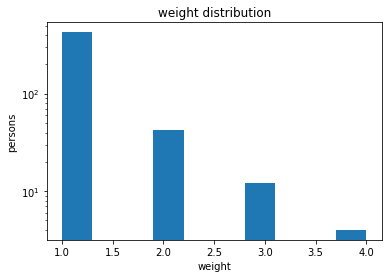
\includegraphics[height=4cm, width=4cm]{images/weight_d.png}
           \column{0.55\linewidth}
              \textbf{Most dangerous concept}\\ \begin{itemize}
                  \item Degree centrality
                  \item Betweenness centrality
                  \item Closeness centrality
                  \item Page Rank centrality
                  \item Eigenvector centrality
              \end{itemize}
              
             Tutte le misure considerate tengono conto dei pesi degli archi.
         \end{columns} 

\end{frame}

%------------------------------------------------

\section{Analisi delle misure di centralità}

\begin{frame}
\frametitle{Analisi delle misure di centralità}
\framesubtitle{Degree Centrality}
\begin{columns}
          \column{0.5\linewidth}
             \centering
             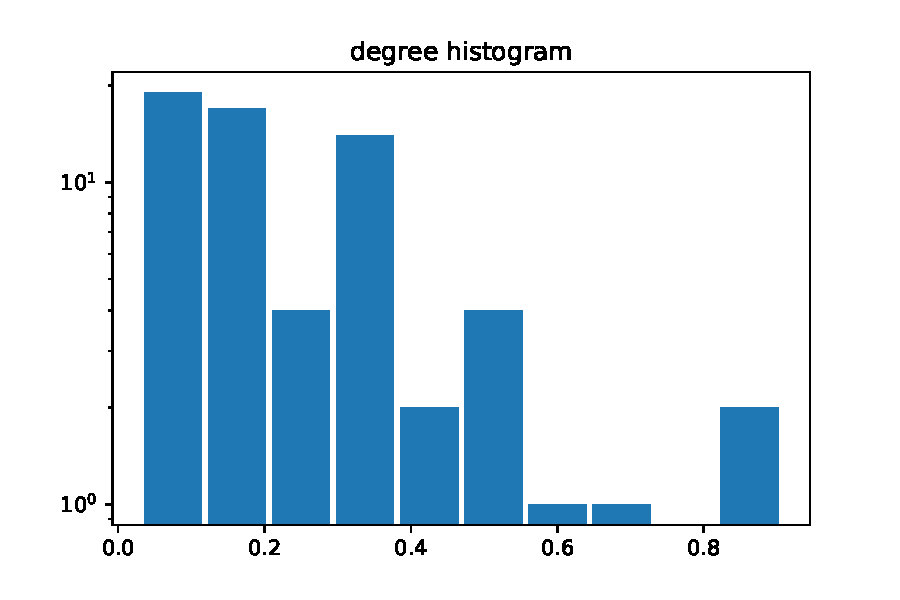
\includegraphics[height=4cm, 
             width=4cm]{images/centrality_measures/degree.pdf}
           \column{0.55\linewidth}
              Questa misura di centralità indica il numero di persone che possono essere raggiunte direttamente da questa persona o può essere interpretata come un indicatore del numero di persone con le quali questa persona si relaziona in modo diretto. 
         \end{columns} 

\end{frame}

%------------------------------------------------

\begin{frame}
\frametitle{Analisi delle misure di centralità}
\framesubtitle{Betweenness Centrality}
\begin{columns}
          \column{0.5\linewidth}
             \centering
             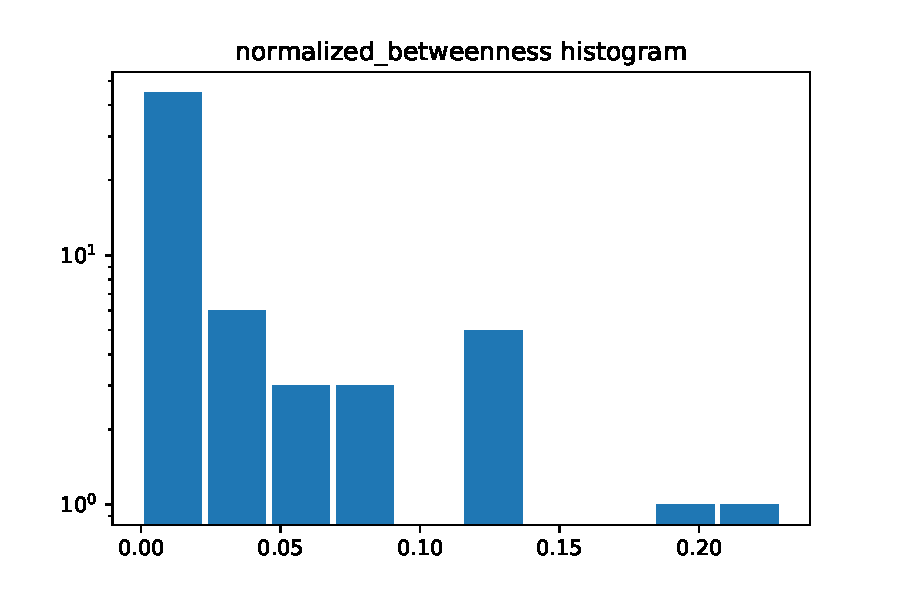
\includegraphics[height=4cm, 
             width=4cm]{images/centrality_measures/normalized_betweenness.pdf}
           \column{0.55\linewidth}
              Questa misura indica l'importanza di una persona rispetto alle volte nelle quali viene utilizzata come ponte da altre coppie di nodi, quindi maggiore sarà il valore associato e maggiore sarà la quantità di informazione a disposizione. 
         \end{columns} 

\end{frame}

%------------------------------------------------

\begin{frame}
\frametitle{Analisi delle misure di centralità}
\framesubtitle{Closeness Centrality}
\begin{columns}
          \column{0.5\linewidth}
             \centering
             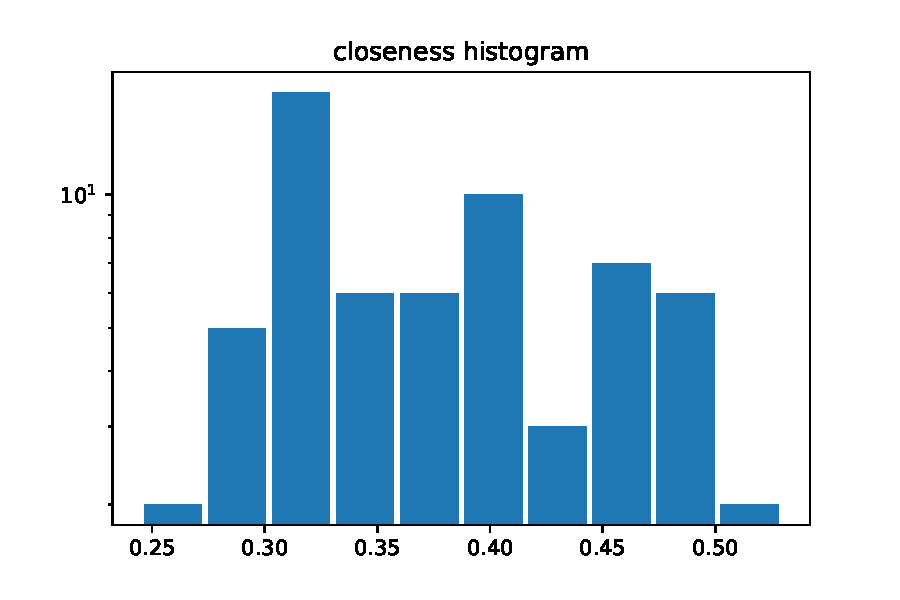
\includegraphics[height=4cm, 
             width=4cm]{images/centrality_measures/closeness.pdf}
           \column{0.55\linewidth}
             Questa misura indica la velocità con la quale una persona riesce a trasmettere certa informazione o interagire con altri nella rete data la sua posizione rispetto alla centralità della rete. 
         \end{columns} 

\end{frame}

%------------------------------------------------
\begin{frame}
\frametitle{Analisi delle misure di centralità}
\framesubtitle{Pagerank Centrality}
\begin{columns}
          \column{0.5\linewidth}
             \centering
             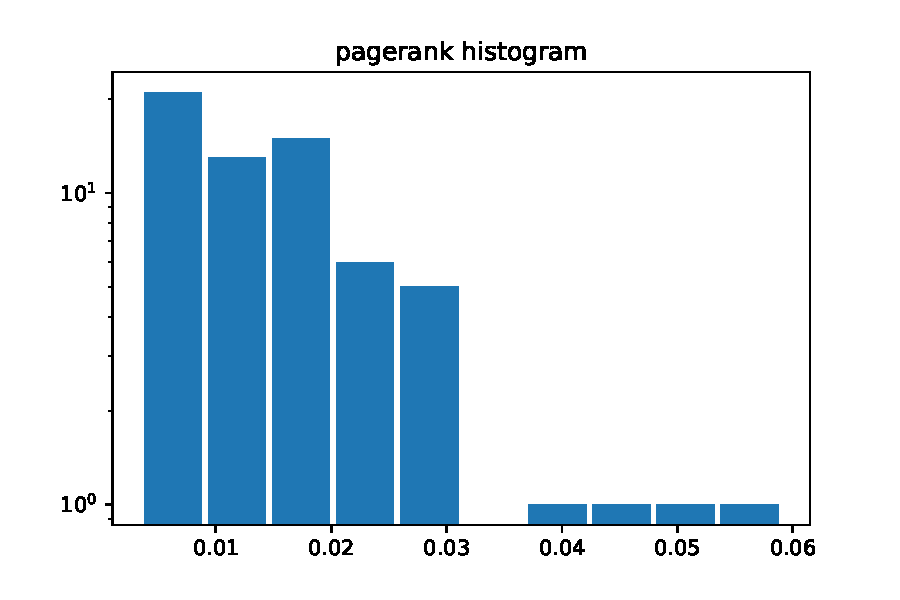
\includegraphics[height=4cm, 
             width=4cm]{images/centrality_measures/pagerank.pdf}
           \column{0.55\linewidth}
       Come EigenCentrality, PageRank può aiutare a scoprire persone influenti o importanti la cui portata si estende oltre le loro connessioni dirette.La principale differenza con EigenCentrality è che il PageRank prende in considerazione la direzione e il peso del collegamento e in considerazione la direzione e il peso del collegamento.
         \end{columns} 

\end{frame}

%------------------------------------------------

\begin{frame}
\frametitle{Analisi delle misure di centralità}
\framesubtitle{Eigenvector Centrality}
\begin{columns}
          \column{0.5\linewidth}
             \centering
             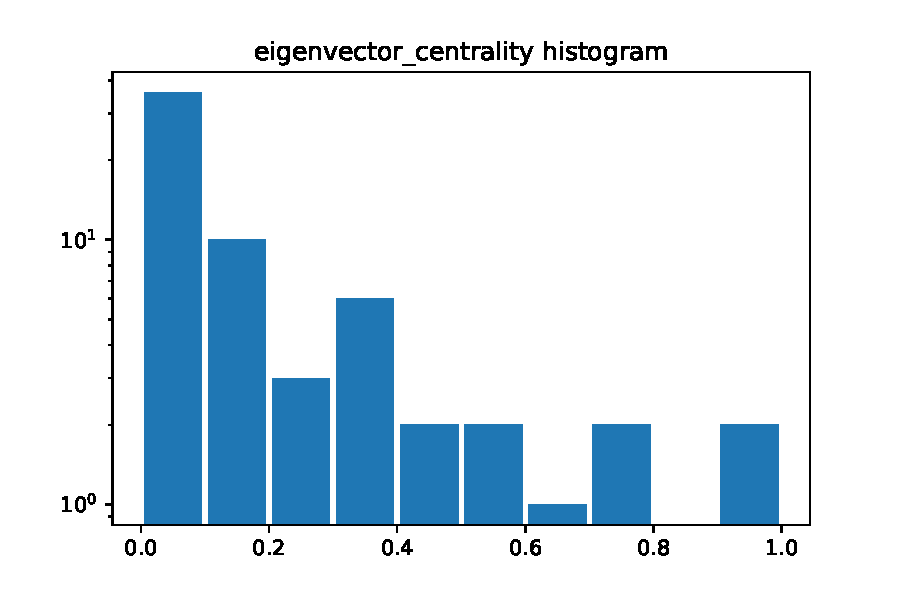
\includegraphics[height=4cm, 
             width=4cm]{images/centrality_measures/eigenvector_centrality.pdf}
             
           \column{0.55\linewidth}
            Questa misura indica quanto una persona è importante rispetto alle persone che la referenziano direttamente. \\
            È utile perché indica non solo l'influenza diretta, ma implica anche l'influenza sui nodi più di un "salto".
         \end{columns} 

\end{frame}

%------------------------------------------------

%\begin{frame}
%\frametitle{Analisi delle misure di centralità}
%\framesubtitle{Confronto delle varie misure di centralità}


%\end{frame}
%------------------------------------------

\begin{frame}
\frametitle{Most Dangerous Persons}
\framesubtitle{Confronto delle varie misure di centralità}
\centering
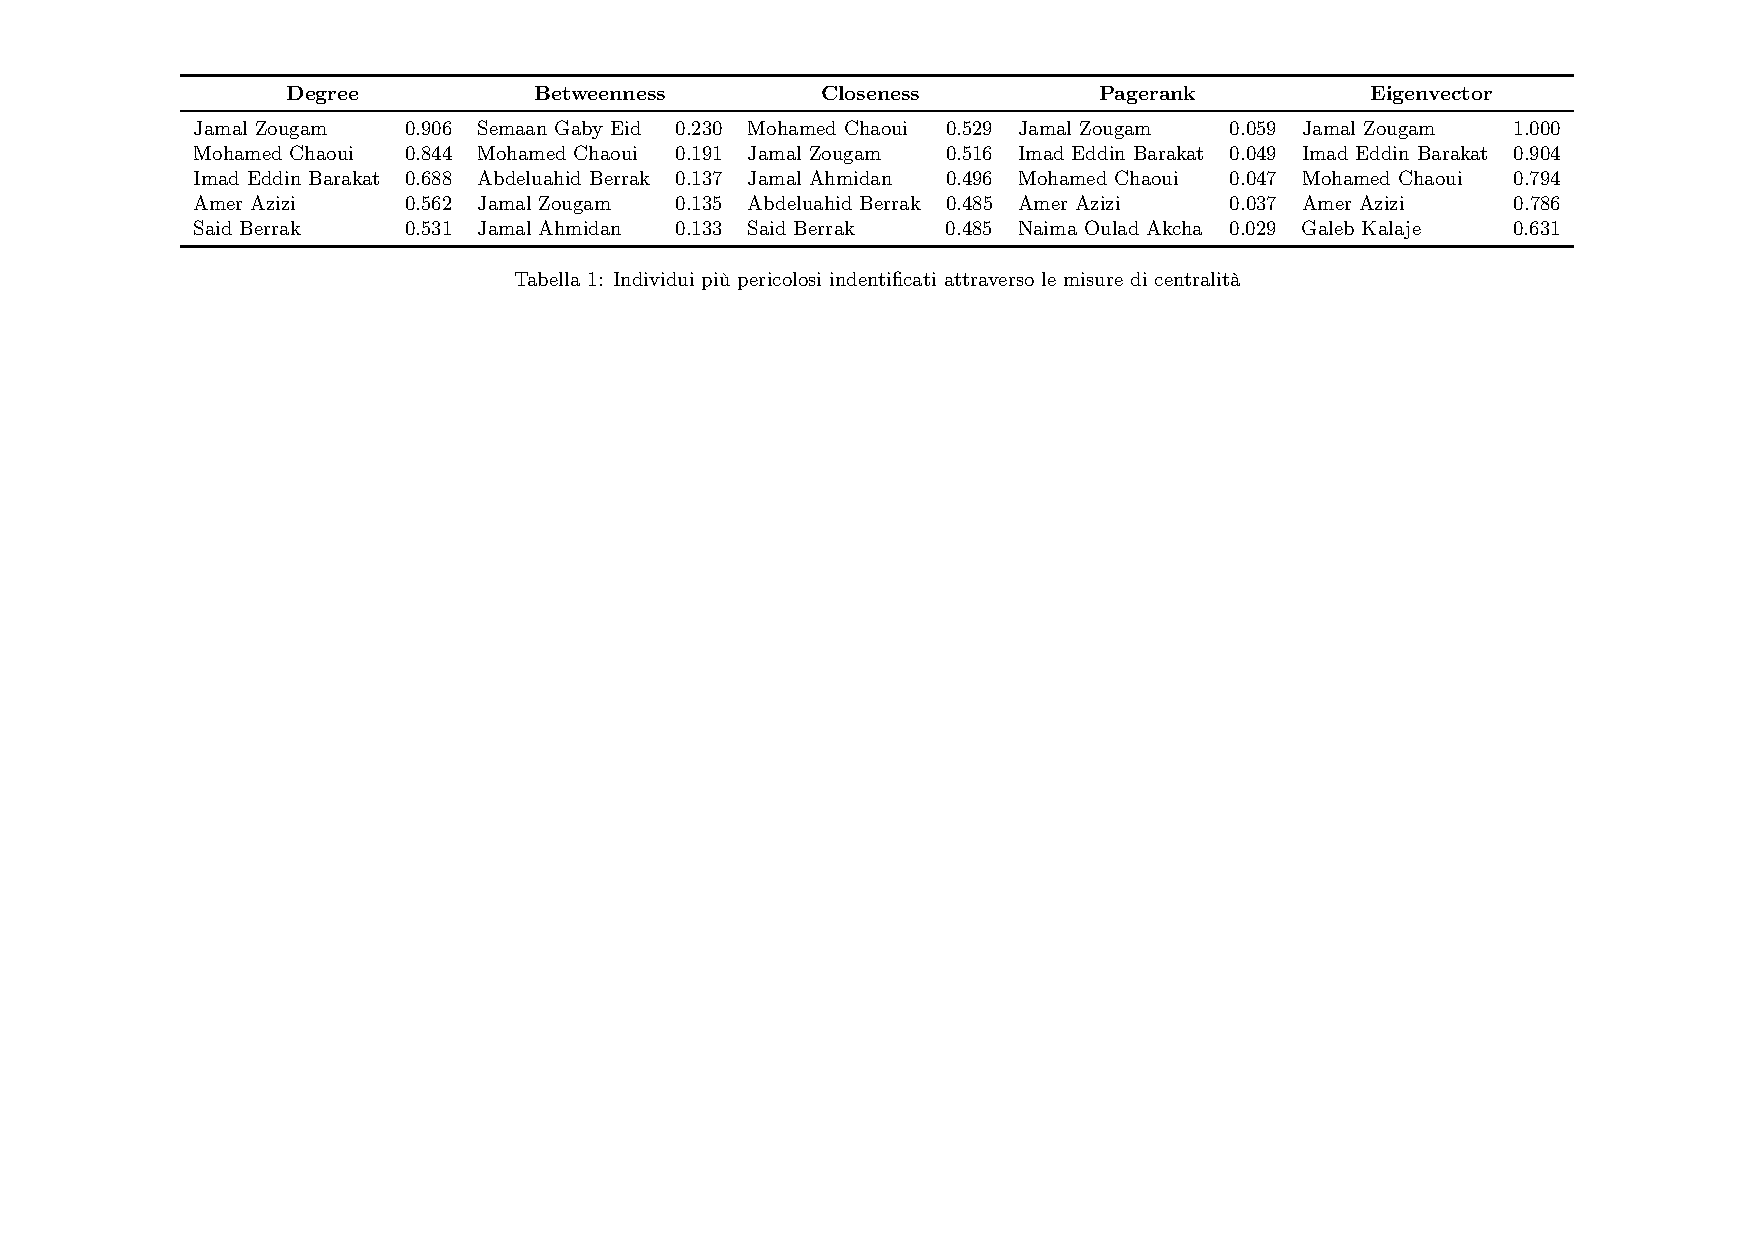
\includegraphics[scale=0.5]{images/most_dangerous.pdf}

\end{frame}
%------------------------------------------------

\section{Community Detection}

\begin{frame}
\frametitle{Community Detection}
\centering
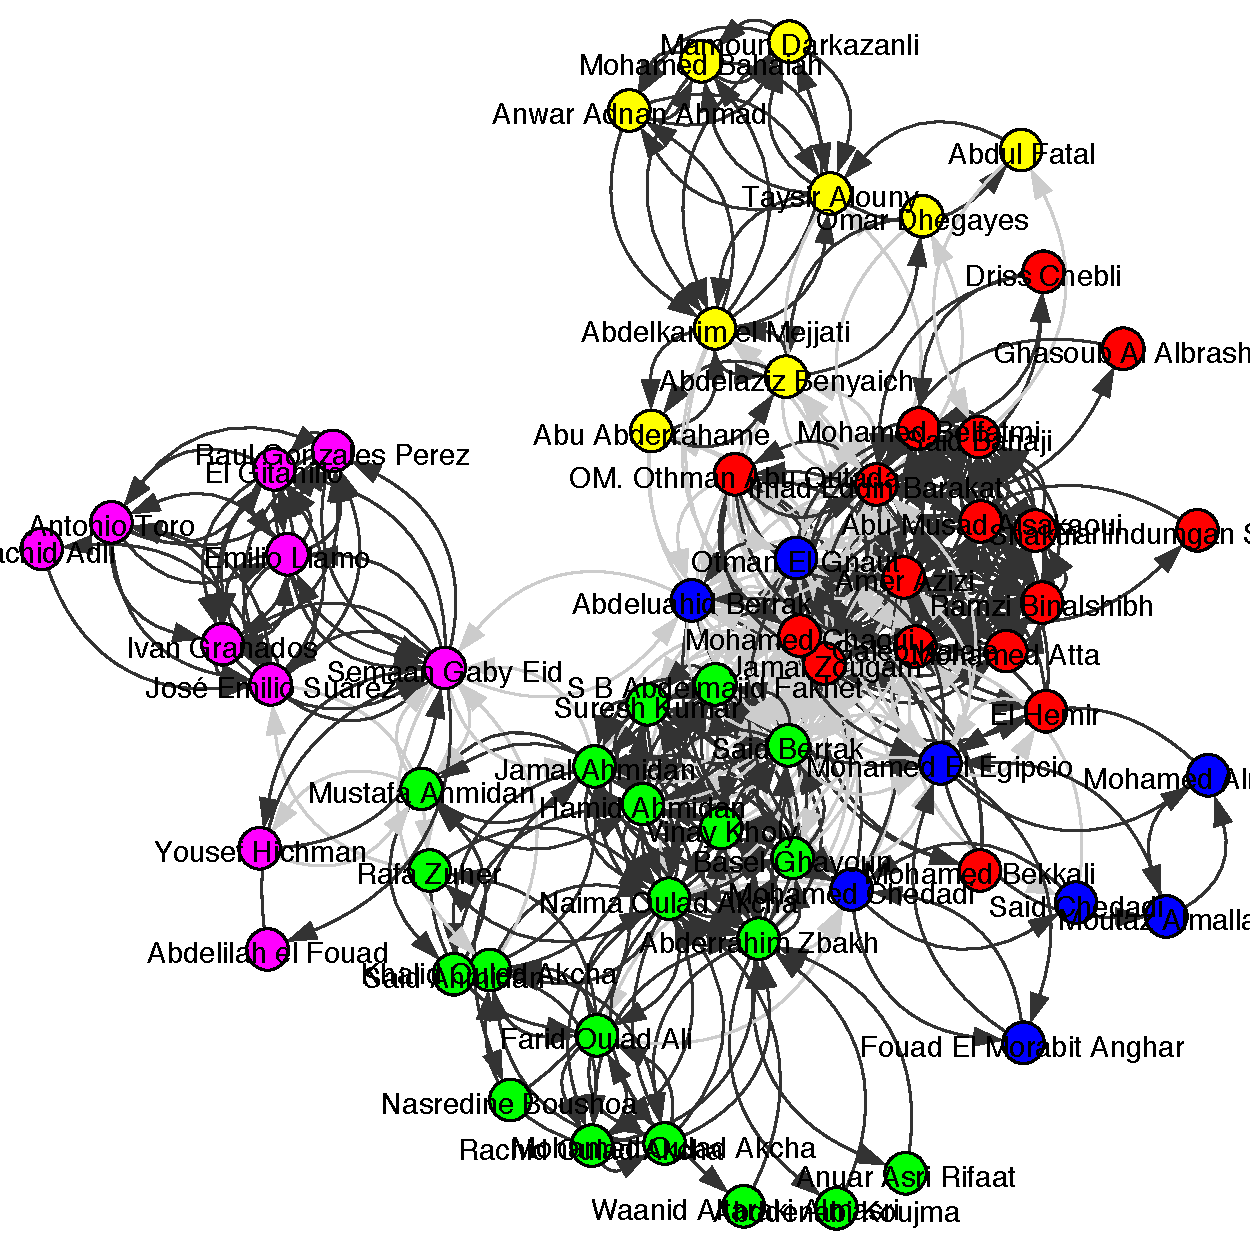
\includegraphics[scale=0.35]{images/community-partition.pdf}
\end{frame}

%------------------------------------------------

\begin{frame}
\frametitle{Community Detection}
\framesubtitle{Confronto delle comunity attraverso le misure di centralità}

\end{frame}

%------------------------------------------------

\begin{frame}
\frametitle{Community Detection}
\framesubtitle{Community Edge Betweenness}
 \centering
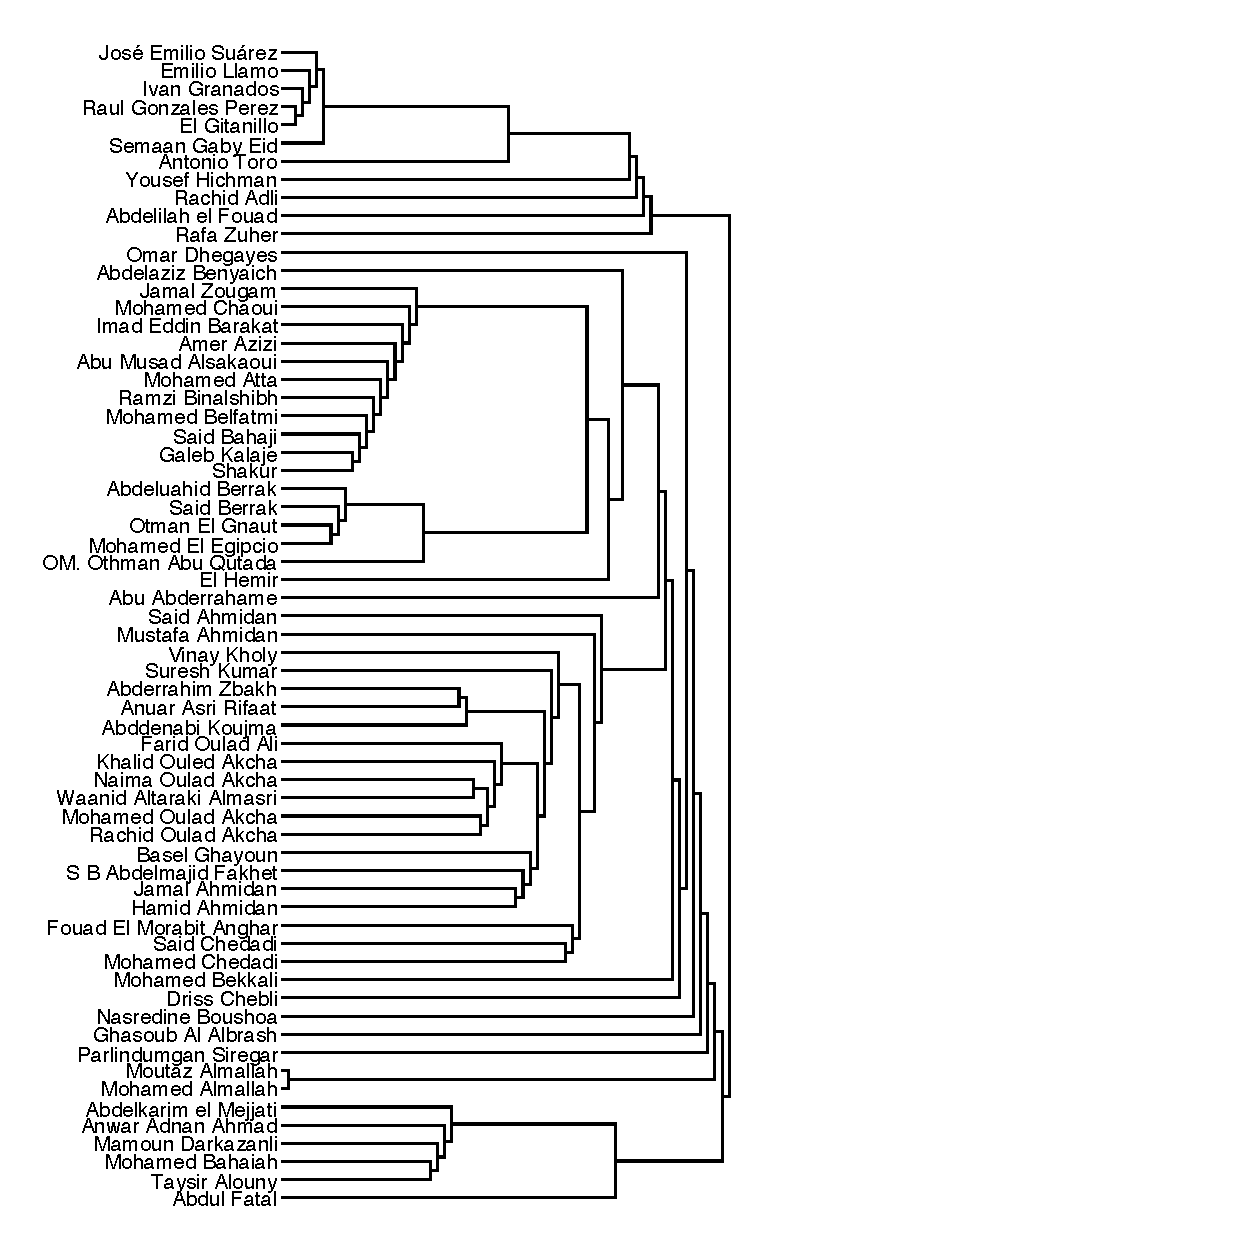
\includegraphics[scale=0.35]{images/community_edge_betweenness.pdf}
\end{frame}

%------------------------------------------------
\begin{frame}
\frametitle{Conclusions}


\end{frame}
%----------------------------------------------

\begin{frame}
\Huge{\centerline{Grazie per l'attenzione}}
\end{frame}

\end{document}
